\chapter{Hardware}

\paragraph*{}
We have encountered issues with reusing old motors and robots from RoboCup Soccer. The Hall effect sensor and the optical sensor have worn out. To address this, we designed and 3D-printed a bracket to mount the Maxon EC 45 Flat motor along with the AS5600 magnetic encoder. We are currently testing the motor to achieve closed-loop control. The motors in the robot are custom-made, and we do not know the number of pole-pairs, making calibration more challenging. We are using the SimpleFOCmini V1.0 drive board, which utilizes the powerful SimpleFOC library for testing.

The next step, after achieving closed-loop control, is to purchase additional motor drivers and control all four wheels. This will allow us to properly drive the X-Drive omnidirectional system using an Arduino, which will then be abstracted to operate under ROS.
\begin{figure}
    \centering
    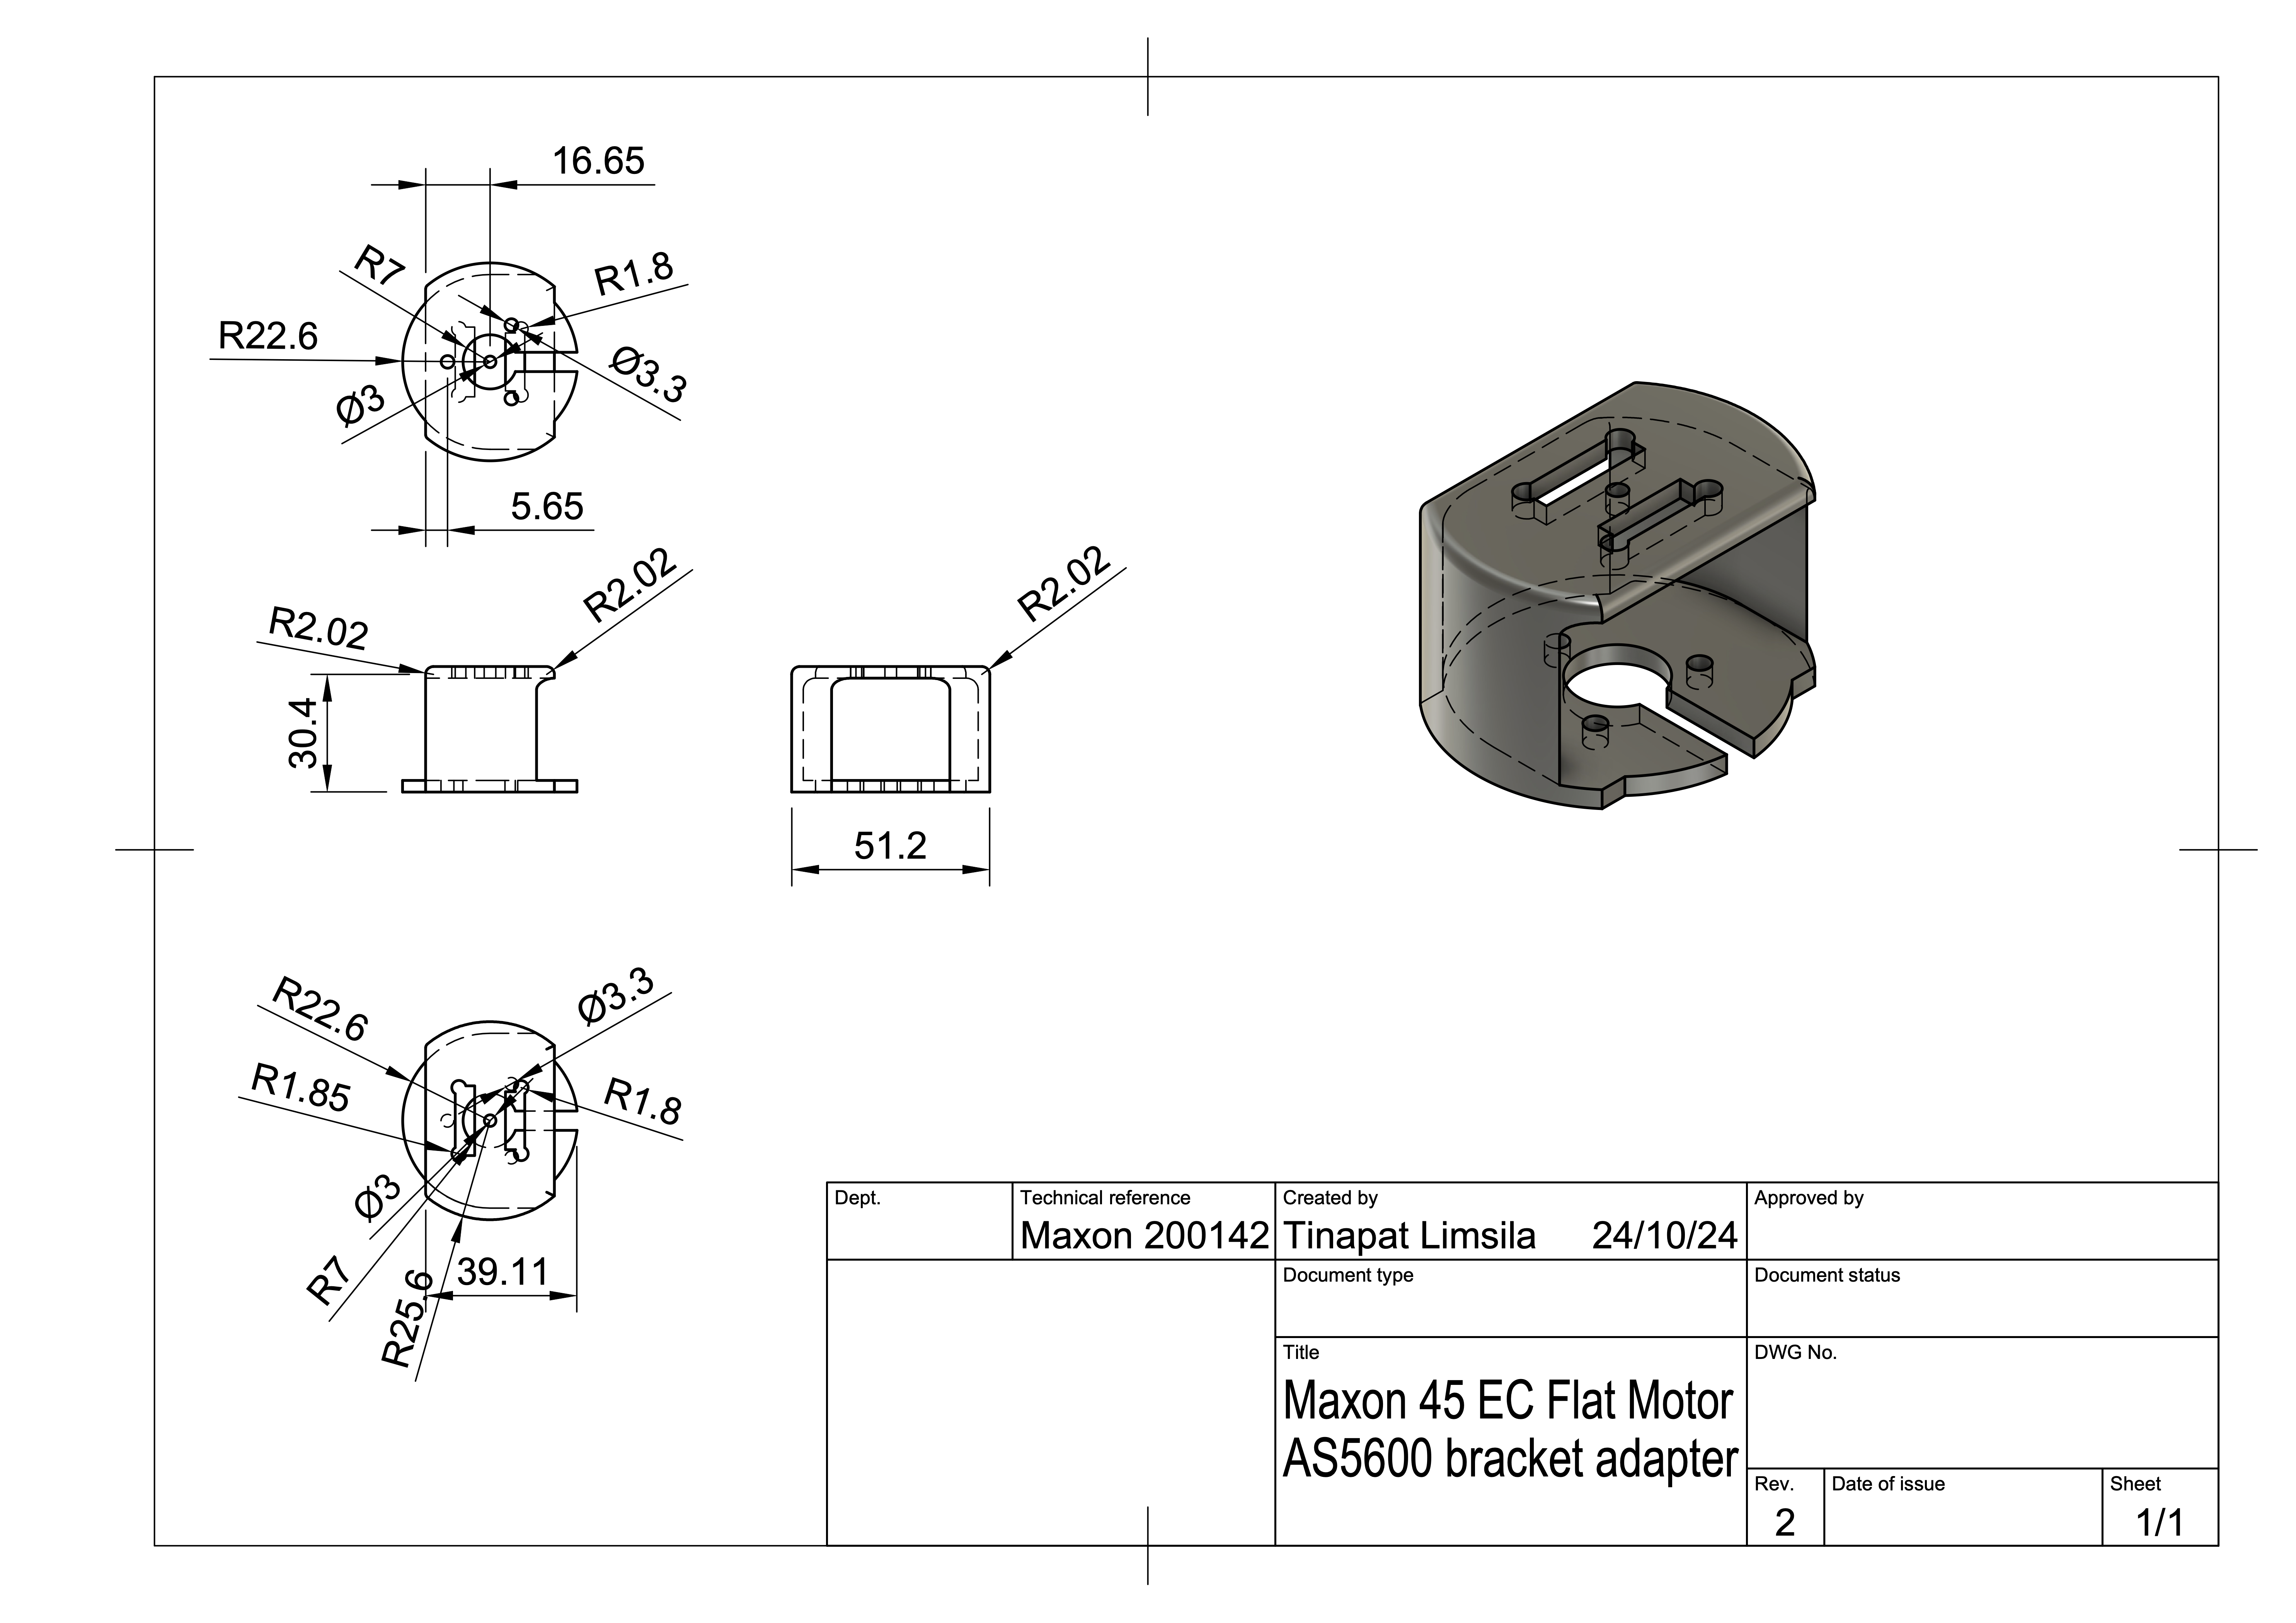
\includegraphics[width=1\linewidth]{Maxon 45 EC Flat Motor AS5600 bracket adapter Drawing v1.png}
    \caption{CAD drawing of the bracket for the Maxon 45 EC Flat motor and the Magnetic Encoder for AS5600}
    \label{fig:enter-label}
\end{figure}